\PassOptionsToPackage{dvispnames, table}{xcolor}
\documentclass[aspectratio=169, hyperref={colorlinks=true}]{beamer}
\usepackage[beamer]{prettytex/base}
\usepackage{prettytex/math}
\usepackage{prettytex/gfx}
\usepackage[backend=biber, citestyle=numeric, bibstyle=numeric, hyperref=true, sorting=none, maxbibnames=99]{biblatex}
\usepackage[toc, acronym, style=long3col, indexonlyfirst=true, nogroupskip=true]{glossaries}
\usepackage{csquotes}
\usepackage{fontawesome}
\addbibresource{../literature/sources.bib}
\renewcommand{\figureloc}{../figures}  % for tikzfigures
\graphicspath{{../figures}}  % for all other figures
\usetheme{oxonian}

\title{General Kernel Spectral Methods for Equilibrium Measures \\ \normalsize Seminar Talk at the University of Graz}
\titlegraphic{
\includegraphics[width=2cm]{../figures/logos/ox-circle.eps}}
\author{Peter Julius Waldert}
\institute{Mathematical Institute \\ University of Oxford}
\date{$9^{\rm th}$ of November, 2023}

\definecolor{lighterOxfordBlue}{RGB}{39, 63, 111}
\definecolor{oxfordGolden}{RGB}{175, 148, 72}
\definecolor{wongGreen}{RGB}{101, 145, 87}
\definecolor{wongPurple}{RGB}{204, 121, 167}
\definecolor{powderBlue}{RGB}{158, 179, 194}
\setbeamercolor{block title}{fg=white, bg=lighterOxfordBlue} % or head
\setbeamercolor{block body}{parent=normal text, bg=lightgrey} % or body, foot
\setbeamercolor{alerted text}{fg=wongGreen}
\renewcommand{\operatorcolor}{lighterOxfordBlue}

\makenoidxglossaries
\newacronym{ml}{ML}{Machine Learning}
\newacronym{gd}{GD}{Gradient Descent}
\newacronym{gui}{GUI}{Graphical User Interface}
\newacronym{lru}{LRU}{Least Recently Used}
\newacronym{pde}{PDE}{Partial Differential Equation}
\newacronym{ad}{AD}{Automatic Differentiation}

\usepackage{xifthen}
\newcommand{\name}[1]{\textsc{#1}}
\newcommand{\inv}{^{-1}}
\newcommand{\qRq}{\quad\Rightarrow\quad}
\newcommand{\qLRq}{\quad\Leftrightarrow\quad}
\newcommand{\functionspace}{L}
\newcommand{\functionspacehat}{\hat{L}}
\renewcommand{\norm}[1]{\left\lVert#1\right\rVert_{\scriptscriptstyle 2}}
\newcommand{\jacobiarg}[1]{2 \norm{\vec{#1}}^2 - 1}
\newcommand{\jacobi}[2][]{P_{\ifthenelse{\isempty{#1}}{k}{#1}}^{(a, b)}\left(\jacobiarg{#2}\right)}
\newcommand{\jacobivec}[1]{\vec{P}^{(a, b)}\left(\jacobiarg{#1}\right)}
\newcommand{\weight}[2][]{\left(1-\norm{\vec{#2}}^2\right)^{\ifthenelse{\isempty{#1}}{a}{#1}}}
\newcommand{\goesto}{\rightarrow}
\newcommand{\hatvec}[1]{\hat{\vec{#1}}}

\newcommand{\hierKoennteIhreWerbungStehen}{
  \begin{center}
    \bfseries \textcolor{themecolor2}{To be done / included.}
  \end{center}
}


\begin{document}
  {\setbeamertemplate{footline}{}\frame{\titlepage}}

  \begin{frame}{Problem Setting}
    \begin{itemize}
      \item Find the Equilibrium Distribution $\rho(\vec{x})$ of a Many-Particle-System.
    \end{itemize}
    \begin{figure}[H]
      \centering
      \begin{subfigure}[t]{0.5\textwidth}
        \centering
        \inputtikz{problem-setting}
        \caption*{$N_p = 8$ particles interacting with one another through the potential $K(r)$.}
      \end{subfigure}
      \hfill
      \begin{subfigure}[t]{0.49\textwidth}
        \centering
        \scalebox{0.68}{\inputtikz{potential-function}}
        \caption*{Plot of attractive-repulsive potential functions $K(r) = \frac{r^\alpha}{\alpha} - \frac{r^\beta}{\beta}$ for different $\alpha, \beta$.}
      \end{subfigure}
    \end{figure}
  \end{frame}

  {
  \setbeamertemplate{footline}{}
  \begin{frame}{Project Motivation and Goal}
    \vspace{0.4cm}
    \begin{itemize}
      \item Model interactions through (power law) attraction-repulsion potentials\footnote{If the repulsive term is stronger (so $\beta > \alpha$), there is no equilibium distribution as particles simply continue repelling each other out to infinity.}
            $$\text{for example,}~K(r) = \frac{r^\alpha}{\alpha} - \frac{r^\beta}{\beta}\quad \text{ with parameters } \quad \alpha, \beta \in \R \backslash \{0\}\,.$$
      \item Each particle $i=1, ..., N$ at position $\vec{x_i} \in \R^d$ and time $t \in \R^+$ follows
            $$\frac{\dd^2 \vec{x_i}}{\ddt^2} = f\left(\norm{\frac{\dd \vec{x_i}}{\ddt}}\right) \frac{\dd\vec{x_i}}{\ddt} - \frac{1}{N} \sum_{j=1, i\neq j}^{N} \nabla K\left(\norm{\vec{x_i} - \vec{x_j}}\right)\,,$$
            for reference see, for example, \parencite{2020-power-law-kernels, 2021-arbitrary-dimensions}.
            For now, we only consider the case without an external potential $V(\vec{x})$.
    \end{itemize}
  \end{frame}
  }

  \begin{frame}{Various Interaction Potentials}
    \begin{figure}[H]
      \centering
      \scalebox{0.8}{\inputtikz{comparing-potentials}}
      \caption[Comparing potentials]{Comparison of different interaction potentials.}
      \label{fig:comparing-potentials}
    \end{figure}
  \end{frame}

  \begin{frame}{Connection to Swarming Behaviour}
    \begin{figure}[H]
      \centering
      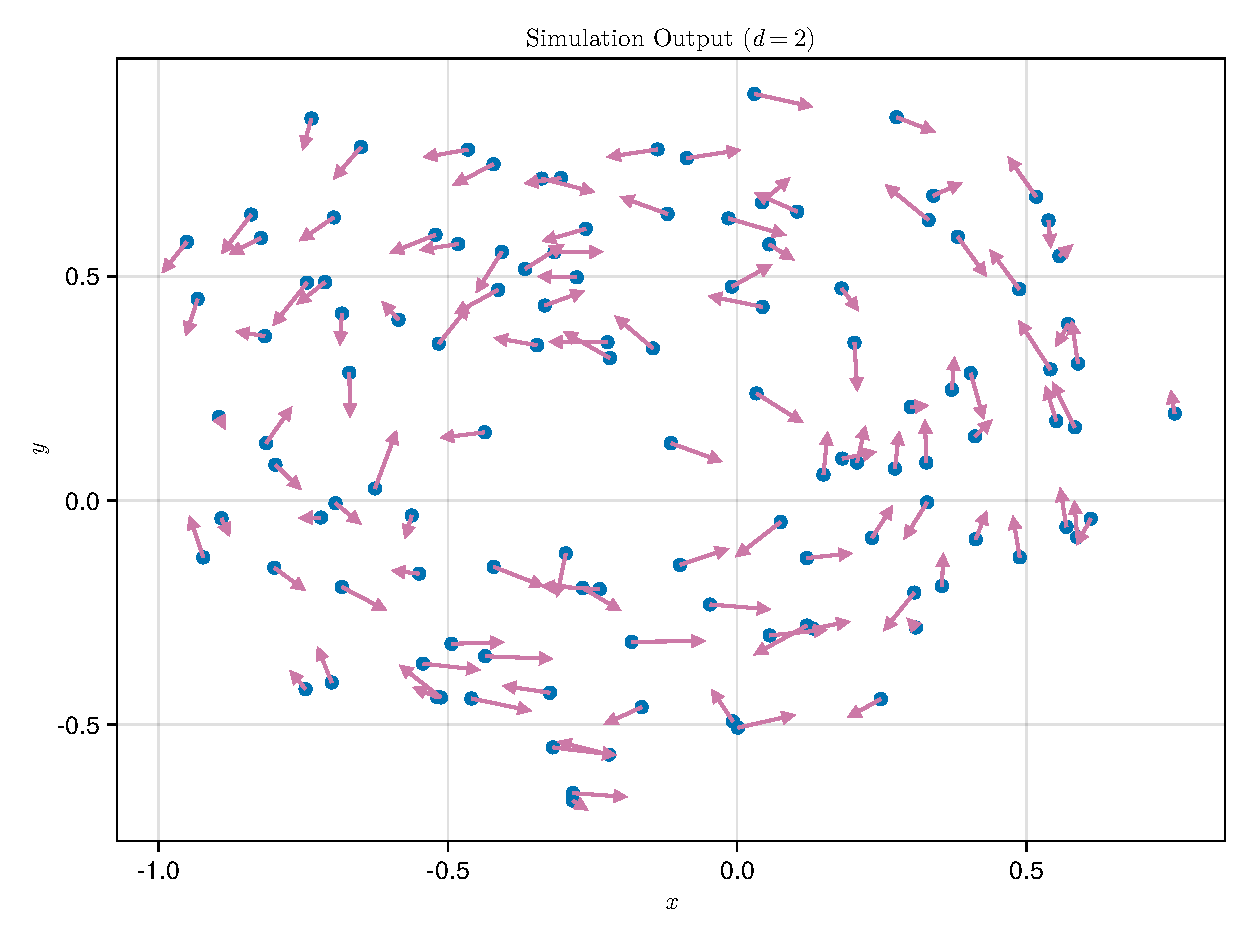
\includegraphics[width=0.56\linewidth]{results/morse-2d/simulation-quiver.pdf}
      \caption[Quiver plot of 120 particles in 2D interacting through the Morse potential]{$N_p = 120$ particles in $d = 2$ dimensions. Morse potential, friction and self-propulsion parameters are as given in \cite{2006-self-propelled}, reproducing their results.}
      \label{fig:simulation-quiver-illustration}
    \end{figure}
  \end{frame}

  \begin{frame}{Leapfrog Integration}
    Every particle $i$ at position $\vec{x_i} \in \R^d$ with velocity $\vec{v_i} \in \R^d$ is updated using
    \begin{align*}
      \vec{x_i}(t+\tau)     & = \vec{x_i}(t)+\tau \cdot \vec{v_i}(t+\tau / 2),              & \quad\text{for}~ & t=0, \tau, \ldots\,,      \\
      \vec{v_i}(t+\tau / 2) & = \vec{v_i}(t-\tau/2) + \tau \cdot \vec{f}[\vec{x_i}(t), t],  & \quad\text{for}~ & t=\tau, 2 \tau, \ldots\,, \\
      \vec{v_i}(\tau / 2)   & = \vec{v_i}(0)+\frac{\tau}{2} \cdot \vec{f}[\vec{x_i}(0), 0], & \quad\text{for}~ & t=0\,,
    \end{align*}
    where $\vec{f_i}[\vec{x_i}(t), t] \in \R^d$ denotes the acceleration (sum of contributions of all forces divided by particle mass $m_i$) at time $t$.
  \end{frame}

  \begin{frame}{Leapfrog Integration}
    In fewer words... a particle at position $\vec{x} \in \R^d$ with velocity $\vec{v} \in \R^d$
    \begin{figure}[H]
      \centering
      \inputtikz{leapfrog}
      \caption[Leapfrog Visualisation]{Visualisation of the Leapfrog integration method, position and velocity are updated at times shifted by $\tau/2$, half the timestep.}
      \label{fig:leapfrog}
    \end{figure}
  \end{frame}

  \begin{frame}{Simulation Demo}
    \begin{figure}
      \centering
      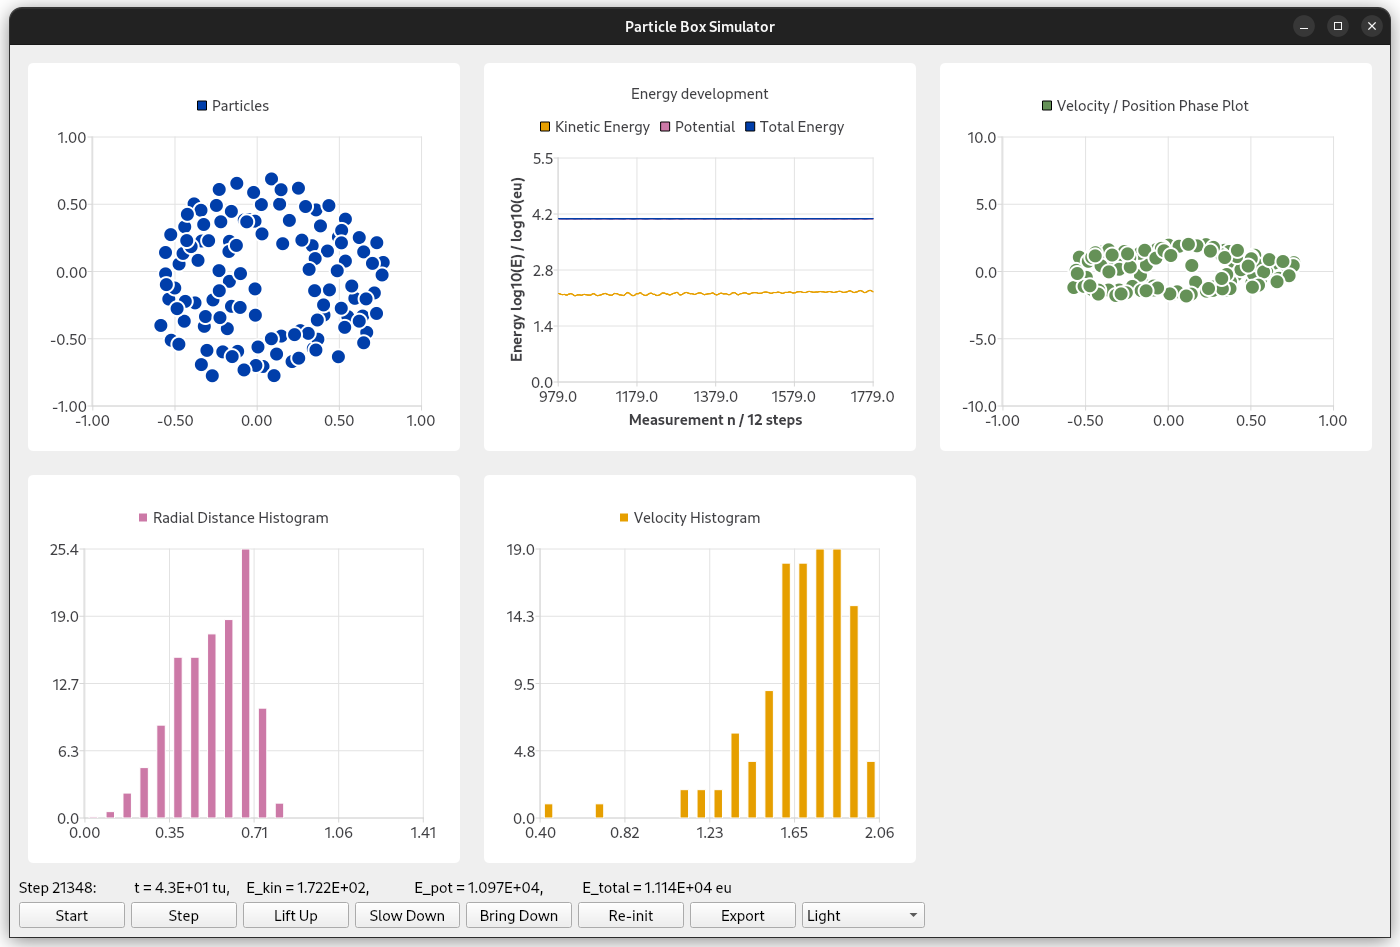
\includegraphics[width=0.64\linewidth]{gui-screenshot.png}
      \caption*{The positional distribution approached by $N_p = 250$ particles.}
    \end{figure}
  \end{frame}

  \begin{frame}{An Integral Equation}
    \vspace{0.4cm}
    The total potential energy of an $N_p$-particle system is then given by
    $$E = \sum_{i=1}^{N_p} \sum_{j=1, j \neq i}^{N_p} K\left(\norm{\vec{x_i} - \vec{x_j}}\right)\,,$$
    which, in the continuous limit as $N_p \goesto \infty$, becomes
    $$E = \frac{1}{2} \iint K\left(\norm{\vec{x} - \vec{y}}\right) \,\dd\rho(\vec{x})\,\dd\rho(\vec{y})\,,$$
    where $\dd\rho = \rho(\vec{x})\dd\vec{x}$ is a measure (the equilibrium distribution) chosen such that
    $$M = \int \dd\rho = \int_{\supp(\rho)} \rho(\vec{x}) \,\dd\vec{x} = 1\,.$$
  \end{frame}

  \begin{frame}{Equilibrium Measures: A Definition}
    \begin{definition}[Equilibrium Measure]
      For a given pairwise interaction potential $K: \R \to \R$, the equilibrium measure $\hat{\rho}: D \to \R$ with $D \subseteq \R^d$ is a measure chosen such that
      $$U_K[\hat{\rho}] := \frac{1}{2} \iint K\left(\norm{\hatvec{x} - \hatvec{y}}\right) \,\dd\hat{\rho}(\hatvec{x})\,\dd\hat{\rho}(\hatvec{y})\,,$$
      is minimised, where $\dd\hat{\rho} = \hat{\rho}(\hatvec{x})\dd\hatvec{x}$ \parencite{2021-arbitrary-dimensions}.
    \end{definition}
    \pause

    For example: in a two-particle system, $\hat{\rho}(\hatvec{x}) = \delta(\hatvec{x}-\hatvec{p_1}) + \delta(\hatvec{x}-\hatvec{p_2})$ to see that
    $U_K[\hat{\rho}] = K(0) + K(\norm{\hatvec{p_1} - \hatvec{p_2}})\,,$
    and hence, the total energy becomes
    $$E = \frac{m}{2} \left(\norm{\hatvec{v_1}}^2 + \norm{\hatvec{v_2}}^2\right) + K(0) + K(\norm{\hatvec{p_1} - \hatvec{p_2}})\,.$$
  \end{frame}

  \begin{frame}{Spectral Methods}
    \begin{itemize}
      \item In order to find $\rho(\vec{x})$, we consider an ansatz of the following form:
            $$\rho(\vec{x}) = \sum_{n=0}^{\infty} c_n \varphi_n(\vec{x})\,,\quad c_n \in \R\,,$$
            with which we construct a spectral method for the numerical solution of the above integral equation.
      \item Minimization routine of $E$ over coefficients in $\rho$, as a subroutine of outer minimisation over the bounds of the box (simpler case: use $[-r, r]$, $r \in \R^+$).
      \item By construction, we find that we do not need an iterative approach for the inner optimisation routine.
      \item The outer minimisation can be performed using known methods from continuous optimisation.
    \end{itemize}
  \end{frame}

  \begin{frame}{Complete Polynomial Basis}
    Jacobi polynomials $P_n^{(a,b)}(x)$ are orthogonal on $[-1,1]$ w.r.t. the weight function
    \begin{equation*}
      w^{(a,b)}(x)=(1-x)^a (1+x)^b\,,
    \end{equation*}
    so they satisfy
    \begin{align*}\label{eq:orthogonalityconditionJacobi}
      \int_{-1}^1(1-x)^a(1+x)^bP_n^{(a,b)}P_m^{(a,b)}\,\ddx = \frac{2^{a+b+1} \Gamma (a+n+1) \Gamma (b+n+1)}{n! (a+b+2 n+1) \Gamma (a+b+n+1)} \delta_{n,m}\,,
    \end{align*}
    with $a	,b>-1$, which uniquely determines $P_n^{(a,b)}(x)$. The special case of $a=b$ corresponds to the ultraspherical or Gegenbauer polynomials, while the case $a=b=0$ corresponds to the Legendre polynomials \cite{2018-nist}.

    \begin{itemize}
      \item This basis yields a \textbf{sparse}, and in particular, \textbf{banded} operator.
    \end{itemize}
  \end{frame}

  \begin{frame}{Summary of the Above / Problem Formulation}
    \begin{definition}[Particle Density Distribution Problem]
      Given an interaction kernel $K: \R^+ \to \R$, the density distribution problem is to find the equilibrium measure $\hat{\rho}: B_R(\vec{0}) \to \R$ of mass $M = 1$ on a $d$-dimensional ball of radius $R \in \R^+$ that minimises the total potential $U_K[\hat{\rho}]$.
    \end{definition}
    \pause

    As mentioned above, we will consider a \alert{spectral method} to solve this problem. More precisely, using the following ansatz:
    \begin{equation}
      \rho(\vec{x}) := \left(1-\norm{\vec{x}}^{2}\right)^{m - \frac{\alpha + d}{2}} \sum_{k=0}^{N-1} \rho_k P_{k}^{\left(m - \frac{\alpha + d}{2},\frac{d-2}{2}\right)}\left(2 \norm{\vec{x}}^{2}-1\right)\,,
      \label{eq:ansatz}
    \end{equation}
    with $P_k^{(a, b)}$ the $k$th Jacobi polynomial and $\rho_k$ its corresponding coefficient.
  \end{frame}

  \begin{frame}{Spectral Method Operator}
    \begin{definition}[Power Law Operator $\mathcal{Q}^\beta$]
      The power law operator $\mathcal{Q}^\beta: \functionspace \to \functionspace$ is given by
      $$\mathcal{Q}^\beta[\rho](\vec{x}) := \int \norm{\vec{x}-\vec{y}}^\beta \,\dd\rho(\vec{y}) = \int_{\supp(\rho)} \norm{\vec{x}-\vec{y}}^\beta \rho(\vec{y}) \,\dd\vec{y}\,.$$
    \end{definition}

    Applied to the ansatz given in \eqref{eq:ansatz}, we can evaluate the appearing integrals \alert{explicitly}.
    For the attractive-repulsive interaction kernel $K_{\alpha,\beta}(r) = \frac{r^\alpha}{\alpha} - \frac{r^\beta}{\beta}$, the matrix representation of the operator becomes
    \begin{equation}
      Q_{\alpha, \beta} := \frac{R^{\alpha+d}}{\alpha} Q^\alpha - \frac{R^{\beta+d}}{\beta} Q^\beta\,.
      \label{eq:full-attrep-operator}
    \end{equation}
  \end{frame}

  \begin{frame}{Evaluation of the Integral}
    \begin{theorem}[Power Law Potential of the $n$th Jacobi Polynomial]
      On the $d$-dimensional unit ball $B_1(\vec{0})$ the power law potential, with power $\alpha \in(-d,2+2m-d)$, $m\in\mathbb{N}_0$ and $\beta>-d$, of the $n$th weighted radial Jacobi polynomial $(1-\norm{\vec{y}}^2)^{m-\frac{\alpha+d}{2}}P_n^{\left(m-\frac{\alpha+d}{2},\frac{d-2}{2}\right)}\left(\jacobiarg{y}\right)$ reduces to a Gaussian hypergeometric function as follows:
      \begin{align*}
        I_{m,n}^{\alpha,\beta}(\vec{x}) & = \int_{B_1(\vec{0})} \norm{\vec{x}-\vec{y}}^\beta \left(1-\norm{\vec{y}}^2\right)^{m-\frac{\alpha+d}{2}} P_{n}^{\left(m-\frac{\alpha+d}{2},\frac{d-2}{2}\right)}\left(\jacobiarg{y}\right) \dd\vec{y}                                                                                                                                                                                                             \\
                                        & = \tfrac{\pi ^{d/2} \Gamma \left(1+\frac{\beta}{2}\right) \Gamma \left(\frac{\beta+d}{2}\right) \Gamma \left(m+n-\frac{\alpha+d}{2}+1\right)}{\Gamma \left(\frac{d}{2}\right) \Gamma (n+1) \Gamma \left(\frac{\beta}{2}-n+1\right) \Gamma \left(\frac{\beta-\alpha}{2}+m+n+1\right)}{}_2F_1\left(\begin{matrix}n-\frac{\beta}{2}, -m-n+\frac{\alpha-\beta}{2} \\\frac{d}{2}\end{matrix};\norm{\vec{x}}^2\right)\,.
      \end{align*}
    \end{theorem}
  \end{frame}

  \begin{frame}{Normalisation of Solutions}
    \begin{lemma}[Mass of the Solution]
      For a given solution $\rho: B_1(\vec{0}) \to \R$, its \textit{mass} $M \in \R$ can be evaluated explicitly, provided the appropriate ansatz, an expansion of weighted radial Jacobi polynomials with coefficients $\rho_k$. The \textit{mass} is given by
      \begin{align*}
        M[\rho[\vec{\rho}]] = \int_{\supp(\rho)} \rho(y) \,\ddy = \frac{\pi^{{d/2}}\Gamma (a+1)}{\Gamma \left(a+{d/2}+1\right)}\, \rho_0\,,
      \end{align*}
      so solely depending on the first coefficient $\rho_0$.
    \end{lemma}
  \end{frame}

  \begin{frame}{Analysis: The Attractive-Repulsive Operator}
    \begin{figure}[H]
      \centering
      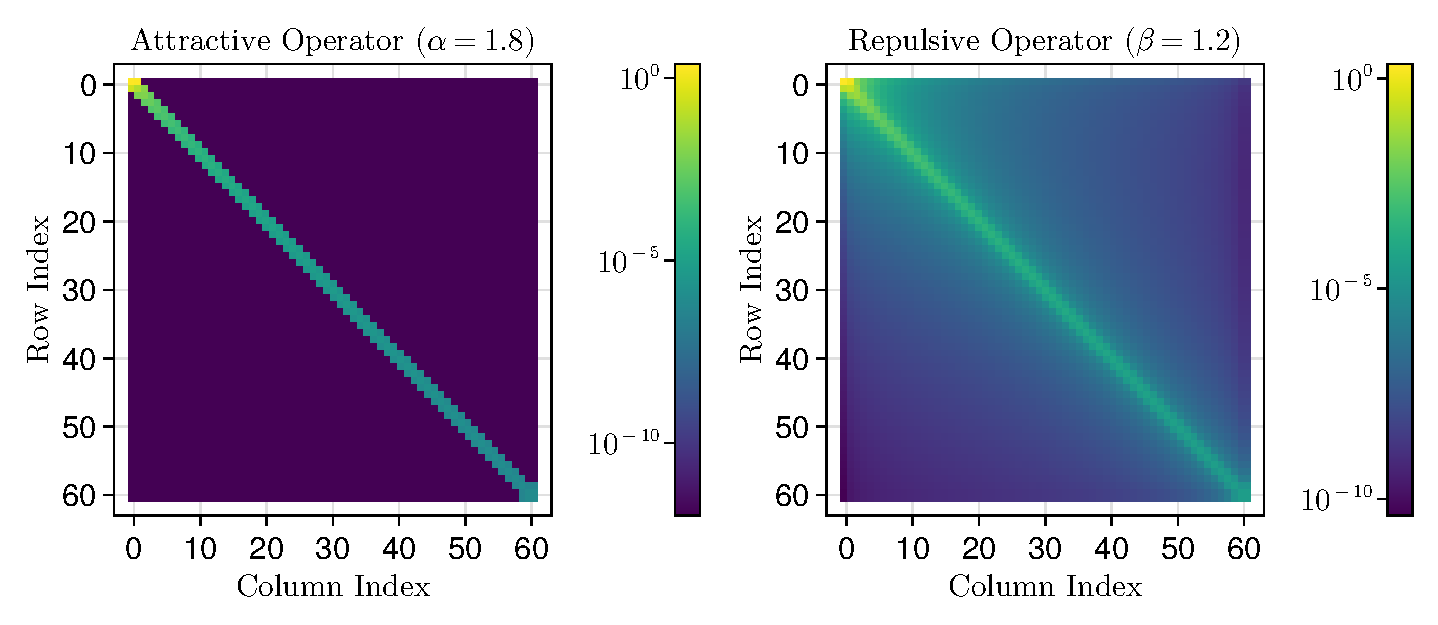
\includegraphics[width=0.9\linewidth]{results/attrep/attractive-repulsive-operators.pdf}
      \caption[Attractive and repulsive operators.]{The attractive and repulsive operators (matrices), the (absolute) matrix values are shown in a $\log_{10}$ colour scale. Due to the choice of basis, the attractive operator is exactly banded.}
      \label{fig:attractive-repulsive}
    \end{figure}
  \end{frame}

  \begin{frame}{Analysis: Comparison with Analytical Solution}
    \begin{columns}[t]
      \begin{column}{0.6\textwidth}
        \begin{figure}[H]
          \centering
          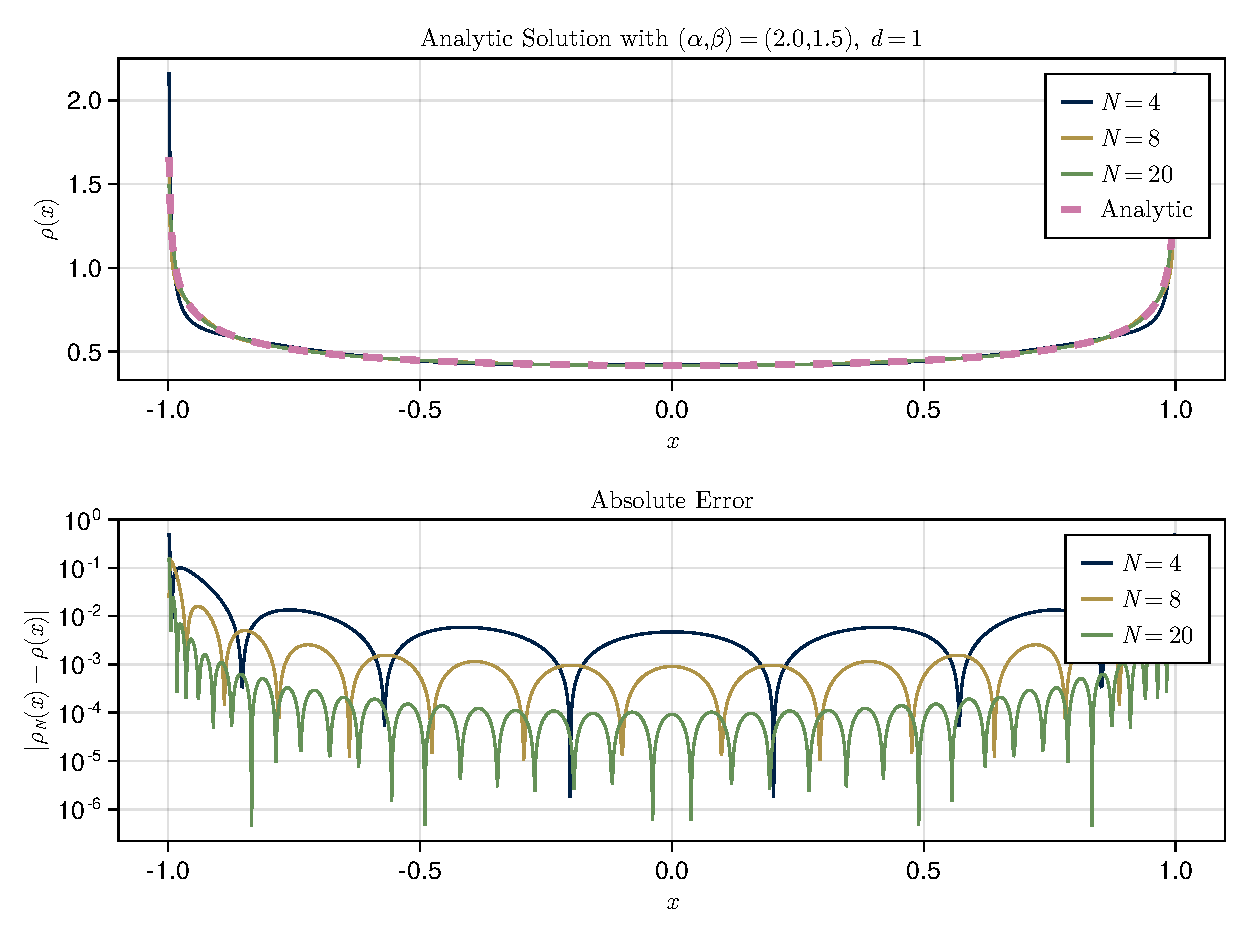
\includegraphics[width=\linewidth, trim={0 6.35cm 0 0}, clip]{results/known-analytic/analytic-solution.pdf}
          \caption[Comparison with analytical solutions and error]{
            The analytical solution $\rho(x)$ compared to the (spectral method) solutions $\rho_N(x)$ of different order.
          }
          \label{fig:analytic-solution}
        \end{figure}
      \end{column}
      \begin{column}{0.4\textwidth}
        \vspace{1.5mm}
        \begin{figure}[H]
          \centering
          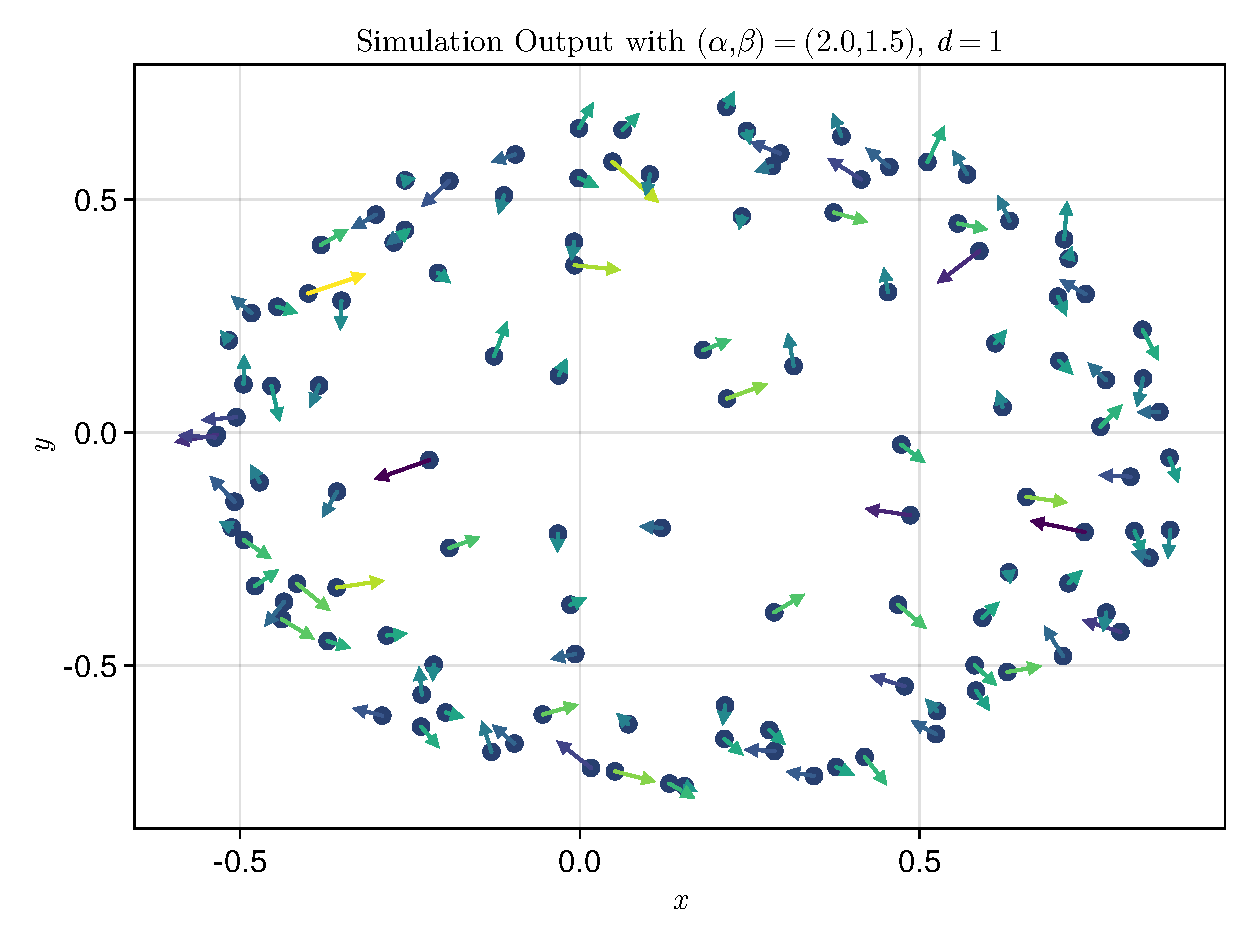
\includegraphics[width=\linewidth]{results/known-analytic/simulation-quiver.pdf}
          \caption[Comparison with analytical solutions and error]{Simulation output with $N_p = 150$ particles using the same attractive-repulsive kernel $K_{\alpha,\beta}(r)$.}
        \end{figure}
        % $$K_{\alpha,\beta}(r) = \frac{r^{2.0}}{2.0} - \frac{r^{1.5}}{1.5}\,.$$
      \end{column}
    \end{columns}
  \end{frame}

  \begin{frame}{General Kernel Spectral Method}
    We express the general kernel as a polynomial, through reprojection from the Jacobi polynomials,
    \begin{equation}
      K_G(r) = \sum_{l=0}^{G-1} g_l r^l \approx K(r)\,,\quad \vec{g} := ({g}_0, ..., {g}_{G-1})^T \in \R^G\,.
      \label{eq:monomial-expansion}
    \end{equation}

    The operator can then be expressed as
    \begin{equation*}
      \mathcal{Q}_G[\hat{\rho}](\hatvec{x})
      = \int_{B_R(\vec{0})} \sum_{l=0}^{G-1} g_l \norm{\hatvec{x}-\hatvec{y}}^l \hat{\rho}(\hatvec{y}) \,\dd\hatvec{y}
      = \sum_{l=0}^{G-1} g_l R^{l+d} \mathcal{Q}^l[\hat{\rho}](\vec{x})\,.
    \end{equation*}
  \end{frame}

  \begin{frame}{Results: Simulation and Solver Comparison}
    \begin{figure}[H]
      \centering
      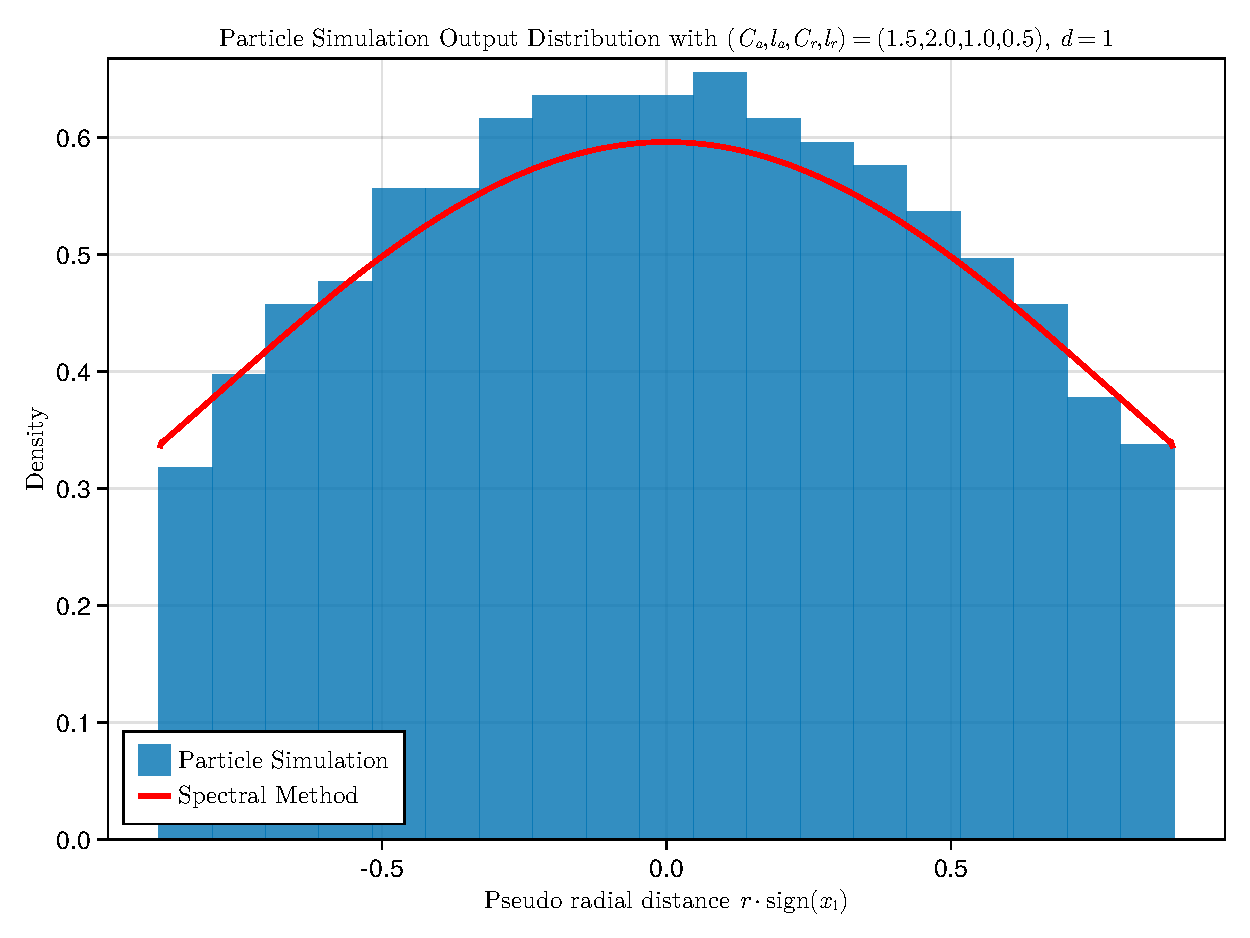
\includegraphics[width=0.58\linewidth]{results/morse/simulation-solver-comparison.pdf}
      \caption[Comparison of histogram and spectral method solution]{Comparison of simulation output with the $G = 8$ general kernel solver's equilibrium measure $\rho_{12}(r)$ at $R$ given by the simulator.}
      \label{fig:simulation-solver-comparison}
      % for now
    \end{figure}
  \end{frame}

  \begin{frame}{Analysis: Well-Conditionedness}
    \begin{figure}[H]
      \centering
      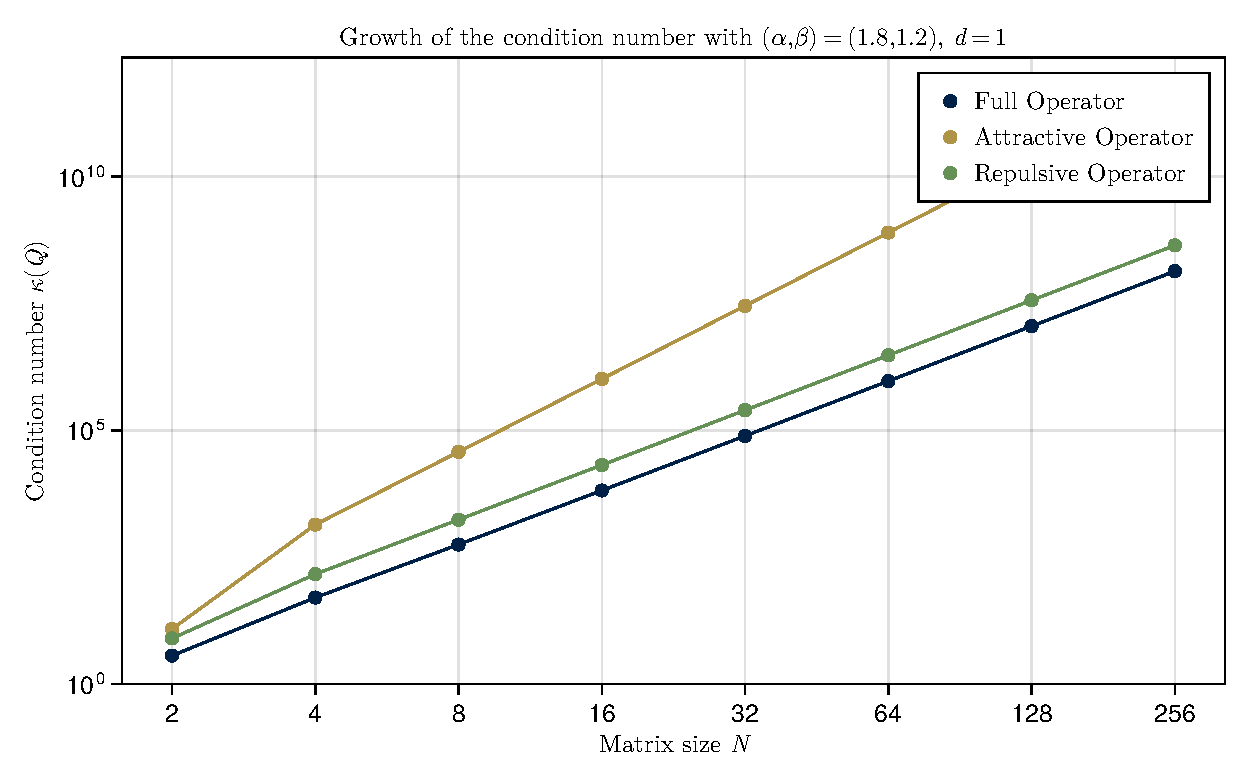
\includegraphics[width=0.65\linewidth]{results/attrep/condition-number-growth.pdf}
      \caption[Growth of the condition number]{Growth of the 2-norm condition number $\kappa_2(Q)$ of the attractive-repulsive operators $Q^{(\alpha)}$, $Q^{(\beta)}$ and $Q_{\alpha,\beta}$ for growing system size $N$.}
      \label{fig:condition-number-growth}
    \end{figure}
  \end{frame}

  \begin{frame}{Analysis: Tikhonov Regularisation}
    \begin{figure}[H]
      \centering
      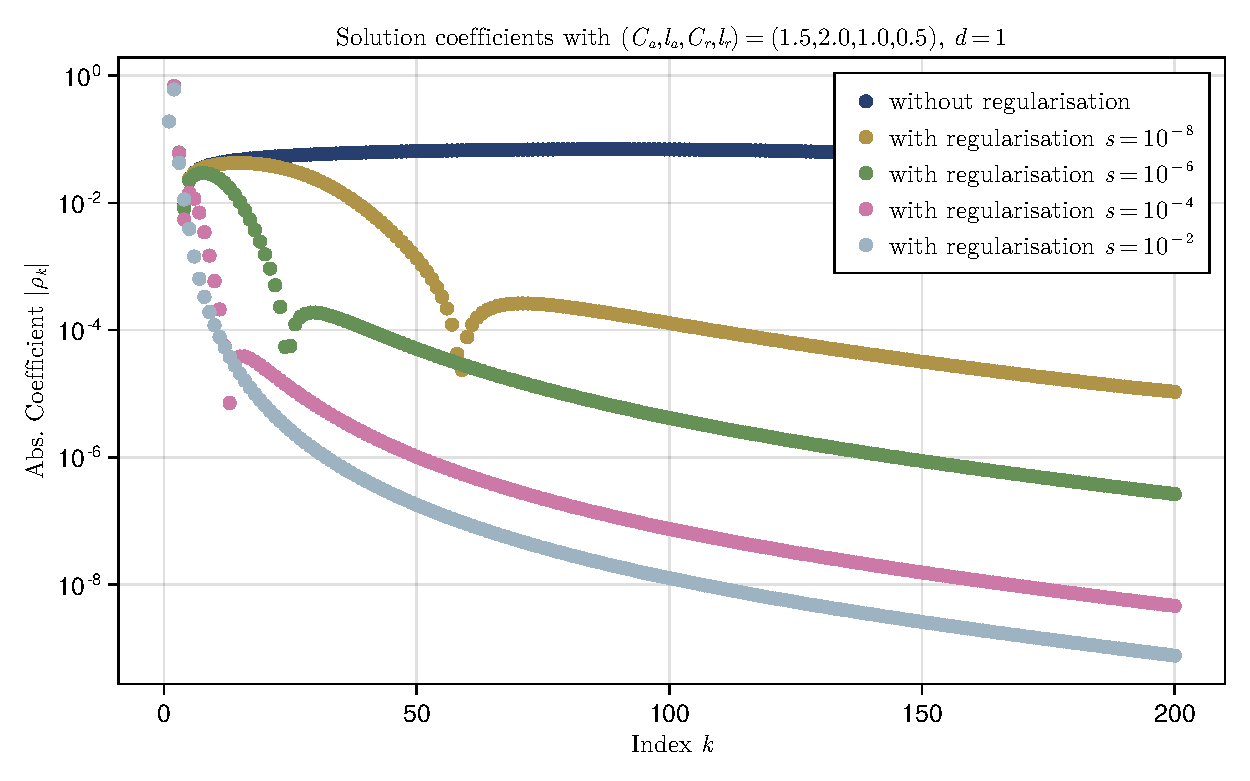
\includegraphics[width=0.65\linewidth]{results/morse/coefficients.pdf}
      \caption[Absolute value of the coefficients with and without regularisation]{Absolute value of the solution coefficients $\rho_k$ with and without Tikhonov regularisation after the solution of a $200 \times 200$ linear system.}
      \label{fig:coefficients}
    \end{figure}
  \end{frame}

  \begin{frame}{Contributions, Challenges Faced \& Future Work}
    Contributions:
    \begin{itemize}
      \tightlist
      \item Original implementation of simulator (+\glstext{gui}, in C++) and solver (in Julia).
      \item General kernel spectral method + implementation.
      \item Lemma for an initial guess of $R$.
    \end{itemize}

    Challenges:
    \begin{itemize}
      \tightlist
      \item Proving Theorem 4.3, the power law integral of the Jacobi polynomials.
      \item Synchronisation of simulation and solver (implementations).
      \item Correct parameter choices for the general kernel spectral method.
    \end{itemize}

    Future Work:
    \begin{itemize}
      \tightlist
      \item Describing phase-space distributions in a self-propulsion setup.
      \item Modelling (constrained) boundaries and boundary conditions.
    \end{itemize}
  \end{frame}

  \begin{frame}{}
    Thank you.
  \end{frame}

  \begin{frame}[allowframebreaks]
    \frametitle{Bibliography}
    \printbibliography[heading=bibnumbered]
    \printnoidxglossary[type=acronym, title={Acronyms}]
  \end{frame}
\end{document}
